\section{Theoretischer Rahmen}
Die Richtlinien zu HCAV nach Lex Fridman sind zumeist auf die Mensch-Maschinen-Schnittstelle bezogen. Da die aufzustellende Wertschöpfungskette Marktwirtschaftliche  Aspekte (Absatz, Marketing, uvm.) integrieren soll, sind mehr Informationen notwendig. So sind Aspekte der Verkaufspsychologie und das generelle Verhalten von Autofahrern zu erläutern. Zusätzlich muss ein Grundwissen zu 'Over-The-Air-Updates' als auch zu Autonomen Fahrzeugen Generell geschaffen werden. Abschließend stelle ich einen essentiellen Baustein der Wertschöpfungskette vor: den SoftwareUser-Pattern-Recognizer [SUPR]. Hierbei zu beachten ist, dass Aspekte des Datenschutzes sowie der Privatsphäre nur im Ansatz beachtet werden.\\
Außerdem stellen wir eine Sammlung an besonderen Situationen und Personas\cite{b99} zusammen um somit nötige Verständnis-Grundlagen für die Bachelorarbeit bereitgestellt zu haben.
\subsection{Der Stand von Autonomem Fahren}
Seit den 1960er Jahren brachte die Automobilbranche Autos auf den Markt, welche immer mehr Fahrtassistenz Systeme hatten. So sind Features wie der Tempomat, das Antiblockiersystem \textit{(ABS)} oder auch der Spurhalteassistent zur Normalität in Neuwagen geworden. Bevor diese Assistenzsysteme jedoch entstanden, musste der Mensch alles alleine unter Kontrolle haben. Neben den Fahrtassistenz Systemen die in die Steuerung mit eingreifen gibt es auch solche, die 'nur' Warntöne oder Lichtsignale auslösen.\\
Im Kontext des Autonomen Fahrens werden Fahrzeuge ihrem Technischen Stand nach in Sechs Stufen aufgeteilt.\cite{b25} In \textbf{Stufe 0} existieren keinerlei automatisierte Fahrfunktionen, sondern nur warnende Systeme die durch aufleuchten und/oder das abspielen von Tönen agiert. In \textbf{Stufe 1} kann das Fahrzeug entweder die Längssteuerung (Beschleunigen/Bremsen) \textbf{oder} die Querführung (Lenken) übernehmen, wobei der Fahrer dauerhaft die jeweils andere Funktion steuert. In \textbf{Stufe 2} kann der Fahrer nun die komplette Steuerung (Längs- und Quer) zeitweilig an das Fahrzeug abgeben. Jedoch muss er in der Lage sein, diese schnellstmöglich wieder zu übernehmen, wenn das Fahrzeug ihm dieses Signalisiert.
Die darauffolgende \textbf{Stufe 3} wird alternativ auch Hoch-Automatisiert genannt und besagt, dass das Fahrzeug die eigenen Fahrmöglichkeiten selber einschätzen kann. Daraus folgt, dass der Fahrer nicht mehr wie in Stufe 2 'schnellst möglich' agieren muss, sondern stattdessen nach einer gewissen Zeitspanne die Steuerung wieder übernehmen muss. In der\textbf{ Stufe 4} kann der Fahrer die komplette Steuerung des Fahrzeugs für bestimmte Anwendungsfälle \textit{(bspw. fahren im Stau)}abgeben. Ist der vom System abgedeckte Anwendungsfall vorbei, übernimmt der Fahrer wieder die Steuerung. Das vollkommen Fahrerlose Fahren wird erst mit \textbf{Stufe 5} realisiert. Hierbei kann das Auto alle möglichen Anwendungsfälle selbstständig abdecken und sich selber komplett steuern. "Wann dieser Automatisierungsgrad erreicht sein wird, kann heute noch nicht benannt werden" (VGL. \cite{b25} Seite 14).\\
Heute hergestellte Fahrzeuge sind technisch in manchen Anwendungsfällen wie bspw. dem selbstständigen Parken bereits auf der Stufe 4 angelangt.\cite{b25} Auch Features der Stufe 3 sind schon vorhanden, wie zum Beispiel das Fahren im Stau und ab naher Zukunft auch das Generelle Fahren auf der Autobahn. Die VDA rechnet damit, dass Autos ab dem Jahr 2030 in der Lage dazu sind, in Innenstädten zu Fahren. Der CEO des bekannten Automobilkonzerns 'Tesla' Elon Musk hingegen sagt, dass ein Tesla schon im Jahr 2020 ein Roboterauto der Stufe 3 oder 4 sein wird.\cite{b28}\\
\\
Ab davon, wann welche Stufe voraussichtlich erreicht wird, stehen viele Menschen Autonomen Fahrzeugen noch immer sehr kritisch gegenüber oder haben ein falsches Verständnis dieser. Genauer gesagt:viele denken, dass autonome Fahrzeuge schon heute unter uns sind.\cite{b31} Die definierten Stufen sind oft unbekannt, hinzu kommen unterschiedliche Meinungen über Social Media, wann die Menschheit die Stufe 5 zuverlässig schafft. Das schnelle, aggressive Tempo des US-Autobauers Tesla hat für das Unterehmen zur Folge, immer wieder Fehler bei bereits verkauften Autos beheben zu müssen \textit{(Metallschäden bei automatischem parken, steigende Zahl der Unfälle in einem Tesla\cite{b32})}. Nichts desto trotzt sind Autonome Fahrzeuge der sicherere Fahrer als der Mensch. Das Auto wird nie Müdigkeitsanfäle haben, nie im Stress sein und deshalb aggressiv fahren, sich immer an die Straßenverkehrsordnung halten und vor allem kann das Auto durch die Vielzahl an Sensoren die komplette Umwelt Millimeter genau wahrnehmen - wozu der Mensch nie in der Lage sein wird. Vor allem für Alte und Kranke stellen Autonome Fahrzeuge eine Möglichkeit dar, wieder mehr Kontakt zur Außenwelt herstellen zu können.\\
Dennoch handelt es sich bei autonomen Fahrzeugen  prinzipiell um keine komplett neue Funktion in unserem Leben. So existiert am Düsseldorfer Flughafen eine Magnetschwebebahn, an fast jeder Ski-Piste finden sich Ski-Lifts und so weiter. Das Fortbewegen passiert bei diesen Systemen auch automatisch und man ist abhängig von einer Maschine. Allerdings greifen wir mit autonomen Fahren in das direkte, alltägliche Umfeld eines jeden Menschen ein. Durch dieses Eindringen in die Privatsphäre, entsteht Angst/Bedenken bei Menschen, da etwas neues, unbekanntes mehr oder minder 'aufgedrängt wird'.
\\
\\
Um aber letzten Endes zu klären, \textbf{wie} ein Auto überhaupt autonom Fahren kann wird hier ein kleiner Einblick in die technische Ebene gegeben. Hierbei nehmen wir den Tesla Model 3 als Beispiel. Es handelt sich hierbei um ein Elektroauto mit wie bereits erwähnt autonomen Fahrfunktionen. Das unten stehende Bild zeigt sechs verschiedene Komponenten des Fahrassistenten des Model 3. \textbf{Nummer 1} ist eine Kamera die am Heck über dem Nummernschild montiert ist. \textbf{Nummer 2 }steht stellvertretend für die 12 Ultraschallsensoren an Bord.
\begin{wrapfigure}{r}{0.65\textwidth}
  \begin{center}
    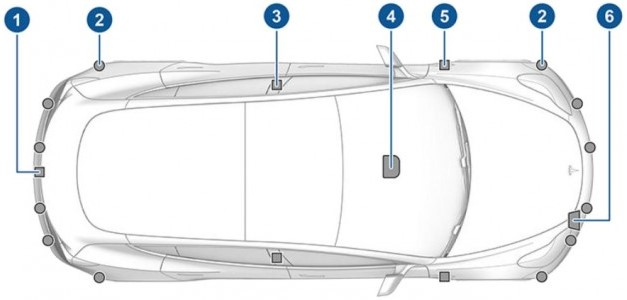
\includegraphics[width=0.63\textwidth]{pictures/tesla2.jpg}
  \end{center}
  \caption{Fahrassistenz Komponenten}
\end{wrapfigure}
\textbf{Nummer 3} ist eine Seitenkamera, gespiegelt auch auf der anderen Seite des Autos. Ein Konstrukt aus Drei Kameras sitzt als \textbf{Nummer 4} auf dem Dach. Außerdem befinden sich bei \textbf{Nummer 5} zwei weitere Kameras \textit{(ebenfalls gespiegelt)} während die \textbf{Nummer 6} ein an der Front installierter Radar Sensor ist.In SUmme sind dies Acht Kameras, 12 Ultraschall-Sensoren und ein Radar-Sensor. Eine alternative aber durchaus umstrittenne Sensortechnologie, die auch für autonome Fahrzeuge verwendet wird, ist der LIDAR\cite{b29}. Der Grund hierfür ist der hohe Preis von LIDAR Sensoren.
Im Auto selber entscheiden von Tesla entwickelte neuronale Netze anhand der aufgenommen Sensordaten, wie sich die Position des Autos ändern muss. Der Innenraum des Model 3 wird dominiert von einem großen Touchbildschirm, welcher als Mensch-Maschine-Schnittstelle fungiert, d.h. dass der Mensch mittels des Bildschirms mit dem Auto Interaggiert.\\
Die Wichtigkeit dieser Schnittstelle ist für ein autonomes Fahrzeug enorm und kann in meinen Augen in Zukunft den Erfolg eines Autos mitbestimmen. Dazu gehört die eigentliche Nutzeroberfläche, aber auch die Licht- und Tonsignale eines Fahrzeugs gehören hierzu. Ein dritter wesentlicher Bereich sind die Mehrwerte die durch Mensch-Maschinen-Interaktion gewonnen werden können. Durch Fahrerbezogene Daten kann ein Auto persönlicher mit Menschen interagieren, von Ihnen lernen und über diesen lernen. Zu derartigen Systemansätzen später mehr in Kapitel \ref{text:supr}.

Neben den installierten Sensoren eines autos gibt es weitere Fahrassistent unterstützende Komponenten welche die Verlässlichkeit, Sicherheit als auch die Umweltfreundlichkeit von AV steigern können.\cite{b30} Eine dieser Komponenten bzw. eher eine Technologie ist die Car2X Kommunikation. Autos sollen mit ihrer Umwelt (d.h. Ampeln, Autos, uvm.) kommunizieren können um so besonders die sicherheitskritische Informationen zu Verfügung zu haben auch wenn die Situation noch nicht im Blickfeld des Autos ist. Auch können so die Wartezeiten an der Ampel können reduziert werden und der Windschatten kann von Autos genutzt werden um so Spritt oder Strom zu sparen. Eine weitere Kompnente an der viele Teilnahmer der Automobilbranche arbeiten sind 3D-Karten für Navigationssysteme. Diese unterstützen eine Millimetergenaue Positionsbestimmung, welche ein Kernelement der Sicherheit ist. Eine Herausforderung bei 3D-Karten ist es, die Karten aktuell, genauer gesagt \textbf{'Live'}, zu halten. "Bei widrigen Umfeldbedingungen wie Schnee, Nebel oder verschmutzter Fahrbahn können Informationen, die nicht vollständig durch die Fahrzeugsensoren erfasst werden, durch Car-to-X-Kommunikation ergänzt werden. Diese stellt somit eine ideale Ergänzung zum automatisierten Fahren dar." \cite{25}


Die Idee: Durch das vermaschen von C2X-Kommunikation und 3D-Karten ist es in der Zukunft möglich, Karten mit Hilfe unserer Fahrzeuge zu aktualisieren.\\
Betrachten wir nun die generelle Architektur eines Autonomen Fahrzeuges, um so ein fundierteres Verständnis zu schaffen. Hierzu ziehen wir eine Grafik heran, welche Jeff Schneider im Rahmen einer Vorlesung am MIT genutzt wurde.\\
\begin{wrapfigure}{l}{0.65\textwidth}
  \begin{center}
    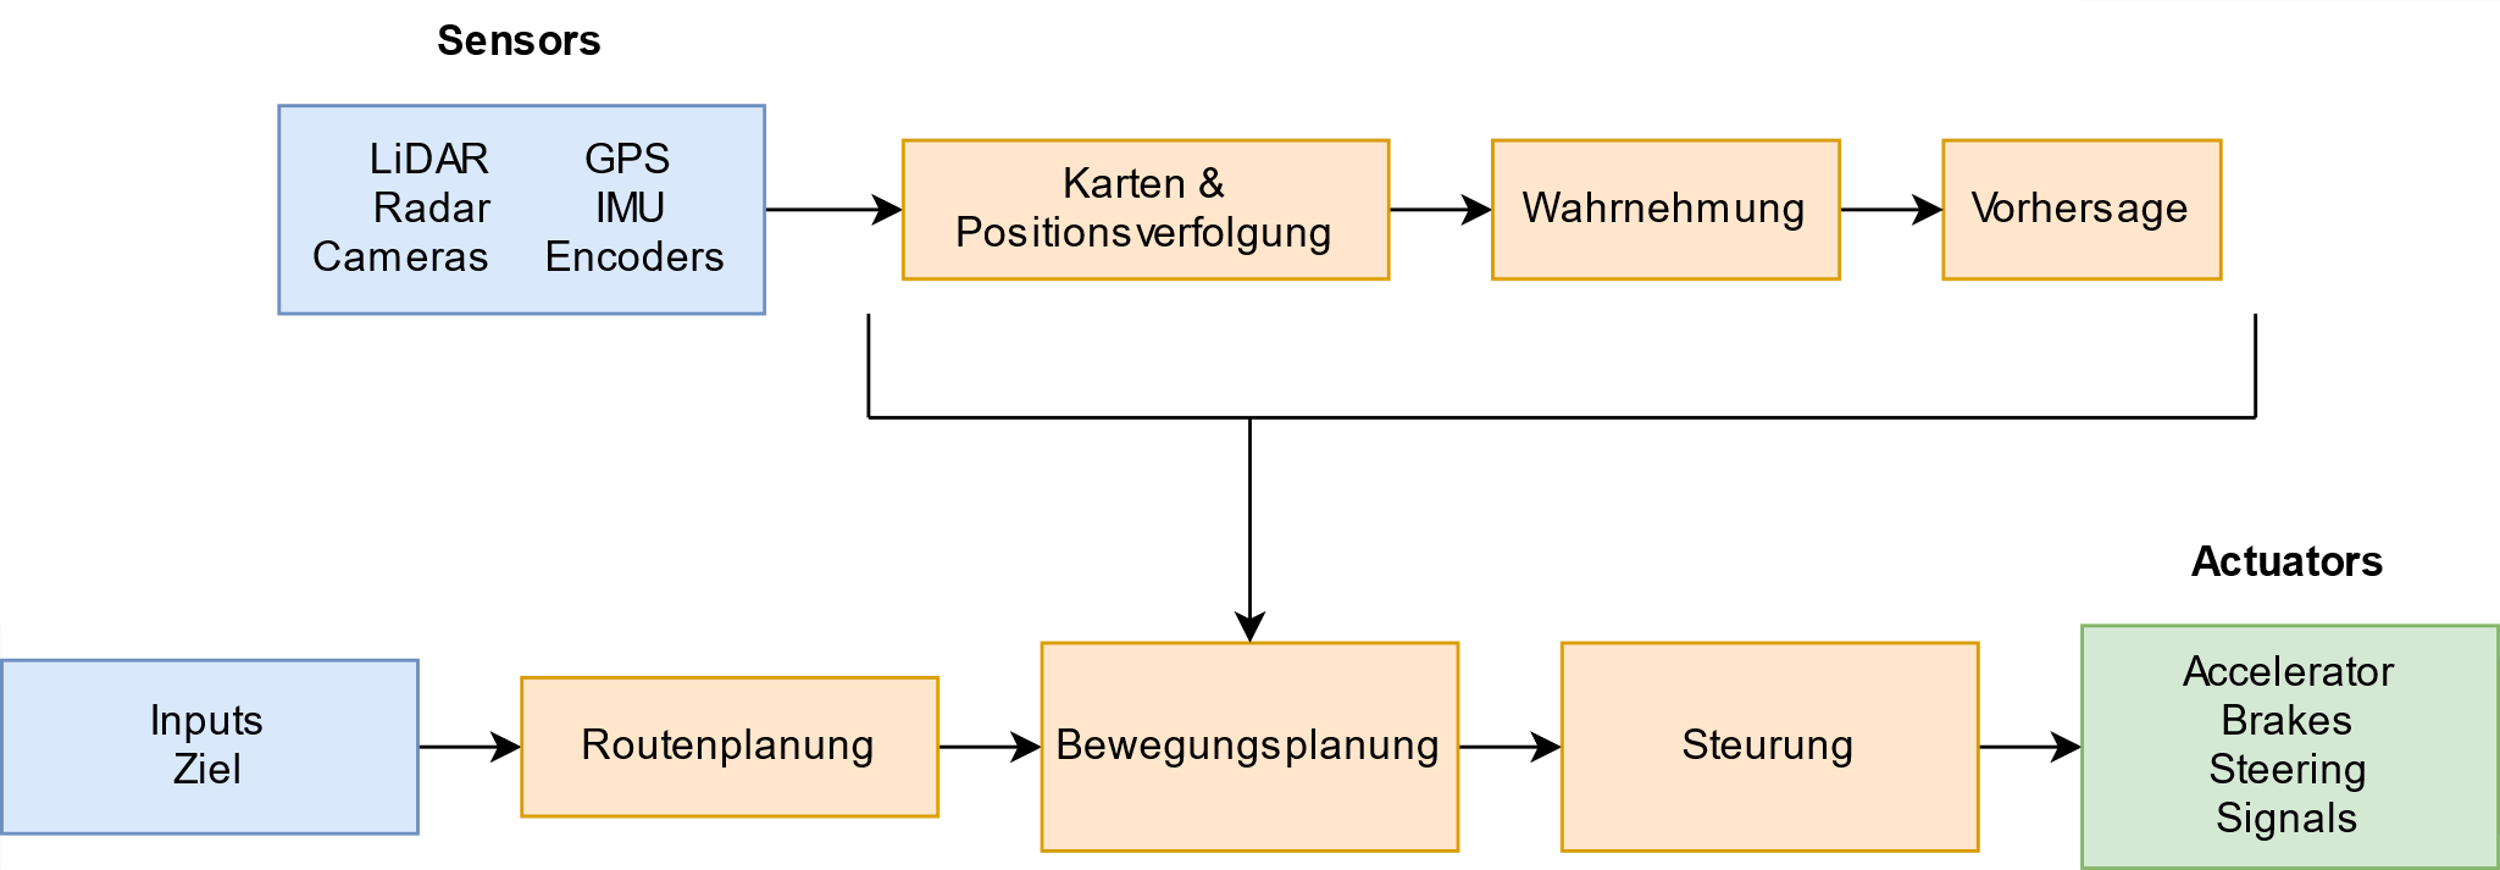
\includegraphics[width=0.63\textwidth]{pictures/arichtecture_AV.png}
  \end{center}
  \caption{Architektur eines AV nach Jeff Schneider}
\end{wrapfigure}
Hier wird verdeutlicht, dass die zuvor besprochenen Sensoren als Input für das Mapping und die Ortung verwendet wird. Es wird also anhand der aufgenommenen Sensordaten  sowie einer 3D-Version der Umwelt die eigene Position bestimmt. Die Wahrnehumng \textit{(Perception)}, identifiziert mit Hilfe neuronaler Netze die anderen Akteure die sich zur Zeit in relevanter Umgebung befinden und ordnet Sie einzelnen Gruppen zu \textit{(d.h. Auto, Passant, Baum, Schild, etc.)}. Die Vorhersage \textit{(Prediction)} bestimmt die verschiedenen möglichen Zukünftigen Routen, die andere Verkehrsteilnehmer fahren könnten. Hierdurch ist das Auto auf alle eventualitäten 
Kostenbasierte analyse, wohinn sich mein Auto als nähstes Bewegt (betrachtet alles aus Maps, Ortung, perception, Prediction und
Über die Karte wissen wir bereits, wo wir überall langfahrne dürfen, wo SPuren hin verlaufen etc 
\\
%Das hier drunter bearbeiten
Tatsächlich ist auch die Gesetzgebung maßgebend für das autonome Fahren. Die Gesetzgeber der einzelnen Länder hängen mit den gestzlichen Vorgaben für Autos oft hinterher, was den Einsatz erschwert.\cite{b20} \cite{b21} So wurde erst \textbf{JAHR EINFÜGEN} das Grundgerüst für autonome Fahrzeuge gelegt, als definiert wurde dass .... gesetzestext nochmal raussuchen. Zusätzlich müssen wichtige Fragen \textit{(Wer ist Schuld an einem Unfall? Wird Insasse wichtiges angesehen als umstehende Lebewesen? uvm.)} vor der weltweiten Einführung geklärt werden.\\
Aktuell ist es so, dass Autohalter für ein Systemupdate in der Regel zu einer Werkstatt fahren müssen. Damit Autonome Fahrzeuge immer die Sicherheit gewähren können, werden sie sich vermutlich mehrmals täglich updaten müssen. Um nicht mehrmals täglich in die Werkstatt zu müssen, forscht die Industrie OTA-Updates \textit{(Over-the-Air)}.
\subsection{Over-the-Air Updates\cite{b33}}
Etwas, was nicht zu vernachlässigen ist, ist die Sicherheit der eingesetzten Software für autonome Fahrzeuge. Neu entwickelte Software hat sehr oft Bugs, wobei ein Software Bug in einem Auto tödliche Folgen haben kann. Hinzu kommt, dass Autos in der Zukunft eine große terroristische Zielscheibe sein werden. Cyberterroristen könnten Fehlfunktionen zu der Software hinzufügen, was ebenfalls tödlich enden kann. Um die Häufigkeit derartiger Aussetzer zu minimieren gilt es, eine sichere Möglichkeit für Updates zu schaffen. Neu entwickelte Software muss am besten beidseitig \textit{(Hersteller und Auto)} verifiziert werden um so gegenüber möglichen Angriffen vorbereitet zu sein.\\\\
Erste Schritte zu einem derartigen System wurden 2010 getätigt, als Justin Samuel, Nick Mathewson, Roger Dingledine und Justin Cappos \textit{"The Update Framework" (TUF)} entwickelten. Dieses bildet den Grundbaustein für das später entwickelte System '\textbf{Uptane}'. Mittlerweile ist es Teil des Automotive Grade Linux Projekts und somit Teil der Linux Foundation. Uptane stellt mittels einer Mehrschichtenarchitektur sicher, dass keine Schädlingssoftware auf ein Auto gelangt. Wie diese Architektur (Abb. 5) designed ist, wird in den kommenden Absätzen dargestellt.\\
\begin{wrapfigure}{r}{0.65\textwidth}
  \begin{center}
    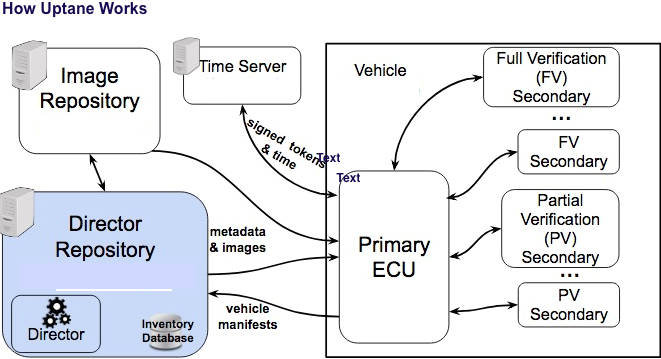
\includegraphics[width=0.65\textwidth]{pictures/uptane_architecture.png}
  \end{center}
  \caption{Architektur Uptane}
\end{wrapfigure}
Es ist vorab wichtig zu erwähnen, dass Uptane lediglich der Standard ist und keine offizielle Implementierung bereitstellt. Beispielhafte Implementierungen wären \hyperlink{https://github.com/advancedtelematic/aktualizr}{aktualizr},
\hyperlink{https://github.com/heartsucker/rust-tuf}{rust-tuf},
\hyperlink{https://github.com/theupdateframework/notary}{Notary} oder 
\hyperlink{https://github.com/advancedtelematic/ota-community-edition/}{OTA Dommunity Edition}.
Kommerziell entwickelte Systeme werden bereitgestellt von \hyperlink{https://www.here.com/products/automotive/ota-technology}{HERE Technologies} und 
\hyperlink{https://www.airbiquity.com/product-offerings/software-and-data-management}{Airbiquity}.\\\\
Die Rechte Seite des Bildes stellen das Fahrzeug dar, während die Elemente zur Linken die Repositories verkörpern. Diese Repositories sind Server und sie haben alle eine eigene wichtige Aufgabe.  Der Time-Server ist dafür da, um ECUs über die aktuelle Zeit zu informieren, da viele ECUs  keine Uhr haben. Das Image Repository speichert jedes derzeit vom OEM verteilte Image zusammen mit den Meta-Daten, welche zur Authentizität benötigt werden. Es nutzt offline Schlüssel um alle metadaten zu 'unterschreiben' bzw. zu verifizieren, was einen hohen Sicherehitsvorteil darstellt. Das Director Repository entscheidet abhängig von den übergebenen Informationen des Autos genau, welche Images an die ECUs verteilt werden müssen. Es nutzt Online Schlüssel zum unterschreiben der Metadaten. Hierdurch haben OEMs die Möglichkeit, schnell neue Software auf den Markt zu bringen. Ein Auto hat mehrere ECUs, welche sich in Speicherplatzgröße, Stromverbrauch und Aufgabenbereich unterscheiden.\\

In dem ersten Schritt eines Updates schickt das Fahrzeug sein Manifest an das Director repository. Dieses enthält informationen darüber, welche Images aktuall auf dem Auto installiert sind. Das Director Repository entscheidet anhand dessen, welche Software auf dem Fahrzeug installiert(geupdated) werden soll. Die Metadaten und die neuen Images werden zurück an die ECU geschickt. Hier findet zunächst eine Verifikation der neuen Images statt, bevor sie anschließend bei Erfolgreichem Test installiert werden. Die Verifikation der ECUs kann entweder vollstöndig oder teilweise erfolgen. \textbf{Vollständig }heißt in diesem Kontext, dass die Größe der Software und die Hashes, welche die ECU über die Metadaten vom Director Repository erhält, identisch sind zu denen
der Metadaten die vom Image Repository zur Verfügung gestellt werden. Bei der \textbf{teilweisen} Verifikation  muss lediglich die Signatur der Metadaten des Director Repositories mit der Signatur der Metadaten vom Image Repository übereinstimmen.
\subsection{Psychologische Aspekte der Verkaufspolitik}
\subsection{Der SoftwareUser Pattern-Recognizer [SUPR]}
\label{text:supr}
Softwarevorschläge, egal ob Fahrfunktion-bezogene oder Feature-bezogene, sollen je nach Insasse individuell bzw. unterschiedlich sein, um möglichst exakt die Interessen der Person(en) zu treffen. Zuzüglich hierzu muss der Zeitpunkt, zu dem eine Software angeboten wird, den Verkauf der SOftware unterstützen, bedeutet: Wenn das Auto eine Software vorzuschlagen hat, soll es hiermit warten bis der Fahrer 'bereit' ist diese zu kaufen. Andernfalls kann der Service von Software Vorschlägen als nervig empfunden werden, was zum einen den Kauf unwahrscheinlicher macht und zum anderen auch das Autonome Fahrzeug an sich in schlechtes Licht rücken wird.\\
Um personalisierte SW-Vorschläge liefern zu können und diese dann zu geeigneten Zeitpunkten anzeigen zu lassen, stelle ich ein Konzept des Software-User Pattern Recognizers (kurz: SUPR) vor. Dieser soll anhand persönlicher Informationen, bereits installierter Software, beliebter Software im (persönlichen) Umfeld und strategisch gestellter Fragen für den Nutzer Sinnvolle Software(Pakete) finden und vorschlagen. Dieser erste Aufgabenbereich ist die \textit{Software Identifizierung}.\\
Der zweite umfasst das \textit{deuten von Gestik, Mimik und Aussagen des Fahrers(bzw. verantwortlicher Person)}, damit auf die Emotion des Fahrers vom System eingegangen werden kann und wichtiger noch eine geeignete Situation für das vorschlagen von SW erkannt werden kann.\\
Durch ein SUPR kann das Fahrzeug stark personalisiert werden. Es kann sich automatisch an die Vorlieben des Fahrers anpassen, heißt Features wie Temperaturanpassung, automatisches Musik abspielen die zur Laune passt, anpassen der Lichtfarbe an Person \& Tageszeit oder auch ein individueller Voice-Assistent(Stimmfarbe, Sprechhäufigkeit, uvm) werden hierdurch ermöglicht. Diese Personalisierung des Fahrzeugs ist der dritte Aufgabenbereich von SUPR.\\
Der 4. und letzte Bereich, der von SUPR abgedeckt werden soll, ist das unterstützen von Nutzereingaben. Wenn etwas wie Routinen im Tages-, Wochen- oder Monatsverlauf festgestellt werden, soll das Fahrzeug bereits auf die zu absolvierenden Strecken vorbereitet sein. Das heißt, dass die Strecke auf mögliche Abschnitte untersucht wird in denen der Fahrer das Steuer übernehmen müsste und für diese Abschnitte geeignete Software gesucht und vorgeschlagen wird.\\
\subsection{Besondere Situationen Sammlung}
Bei Länderwechsel soll sich Auto auf Fahrweise nicht autonomer Fahrzeuge vorbereiten\\
Luxus-Features: Erzählung zu der Region, die aktuell durchfahren wird (Denkmalführungen oÄ.) -> als Luxus SW\\
Software zum kauf: Unterstützen von Blinden/Tauben durch featuresoftware; SOftware, die mein Fahrverhalten kommentiert und auf Fehler meinerseits aufmerksam macht -> kann auch Akzeptanz von AF steiegern, da deren 'genie' gesehen wird; Software zur Parkplatzsuche\\
\subsection{Hinzukommende Richtlinien}
Neben den Richtlinien für das Designen von HCAV sind für meine Arbeit noch weitere Kernelemente immer zu beachten:
\begin{itemize}
	\item \textbf{Verkaufspsychologische Aspekte}\\
	Das von mir zu entwickelnde Konzept umfasst allerdings nicht nur die technische Seite autonomer Fahrzeuge, sondern beschreibt auch mögliche Abläufe zum Softwarevertrieb und -Verteilung. Aufgrund dessen ist es nötig, für das Konzept Verkaufspsychologische Aspekte\cite{b15} einfließen zu lassen.\\
	Wir lassen uns nur ungerne etwas verkaufen, kaufen aber Gerne wenn diese aquirierung bestimmte Wünsche und Bedürfnisse befriedigt. Also: \\
	Schritt 1: herausfinden, was Kunde möchte/will/braucht\\
	Schritt 2: anbieten\\
	Plus- | Chancen- | Minus- Kunden\\
	Bei Einkauf steht der persönliche Nutzen für Kunde im Fokus.\\
	Welche Grundbedürfnisse werden mit welche SW abgedeckt?\\
	Differenzprinzip: unterbewusste Reize setzen, die zum Verkauf leiten; Bei teuerstem Produkt anfangen\\
	Frage ist nicht: 'möchten Sie bei mir kaufen', sondern 'möchten sie Angebot A, B oder C'?\\
	Preise erst beim Verkaufstermin erwähnen\\
	Do-ut-des (Ich gebe, damit du gibst); Gratisproben oÄ, Bei einem Nein: Können sie uns dennoch empfehlen?\\
	2 Schritte vor, einer Zurück Prinzip; schritt 'zurück' erreichen des eigentlichen Ziels (kennt ja keiner außer mir)\\
	Das KonsequenzPrinzip:\\
	Konsequenz im Handeln ist eine positive Charaktereigenschaft\\
	Vorteile und Nachteile von Konsequenz rauschreiben für mich selber (S. 51)\\
	Wenn-Dann-Frage: Wenn wir Ihnen XY bieten können, kaufen sie dann? -> automatische Ticketerstellung möglich für SW-Developer\\
	\begin{figure}[H]
		\centering
		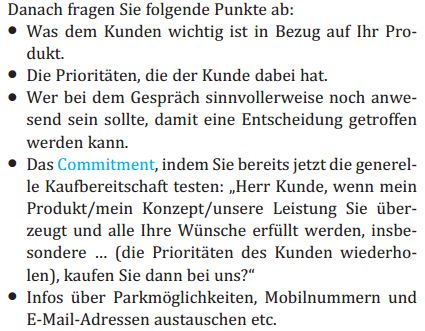
\includegraphics[width=0.734\columnwidth]{pictures/fragenBeiTerminvereinbarung.jpg}
		\caption{bla}
		\label{img:fragenBeiTerminvereinbarung}
	\end{figure}
	Kunden zu einem frühen commitment drängen (wenn-dann)\\
	Welche 'kleinen DInge' kann ich machen, um Kunden vom Kauf zu überzeugen? ->System für diese dinge planen \& Ablauf.\\
	Konsequenzprinzip oft verwenden um einen Fuß in die tür zu kriegen; Nicht unbedingt riesenAuftrag an Land ziehen owllen, sondern erstnmal klein anfangen (kleinvieh macht auch mist)\\
	Umschalten auf 'Autopilot' -> sich den Aktionen anderer Menschen anpassen\\
	Zeugenumlastung: Person lässt sich bestätigen, dass ihr Unternehmen+Produkt gut ist -> andere Menschen zu diesem Gedankengang bringen\\
	Referenztechnik: Von Stammkunden Empfehlungsschreiben holen etc.\\
	Empfehlungsmarketing: Kunden nach Bekannten/(Geschäfts-)Partnern fragen, die Produkt möglicherweise auch haben wollen\\
	Dritte für sich sprechen lassen
	\begin{figure}[H]
		\centering
		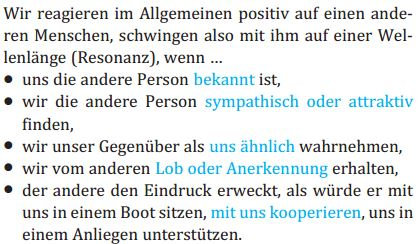
\includegraphics[width=0.734\columnwidth]{pictures/resonanzprinzip.jpg}
		\caption{nix}
		\label{img:resonanzprinzip}
	\end{figure}
	Maskotchen nehmen für Vermittlung von Werbung -> wirkt Vertrauensschaffend und Persönlich\\
	bei unbekannten Neukunden mehr Vertrauen schaffen\\
	Ähnlichkeiten zum Kunden entdecken - dieser fühlt sich dann wohler, was den Verkaufsabschluss leichter gestaltet\\
	\\
	\textbf{Regeln für meinen Anwendungsfall:}
	\begin{itemize}
		\item Den Kunden nicht nerven. Wenn der Kunde 'Kein Interesse' hat, soll eine SW in den Log für vorgeschlagene Software und erst nochmal angeboten werden, wenn der Kunde X mal verwendung für diese SOftware hätte(1. 3 mal, 2. 5 mal usw. oÄ.)
		\item Dem Kunden sollen immer mehrere Angebote zu einer SW gegeben werden (ggf. mit unterschieldichen Features/add ons oÄ)
		\item Den Kunden etwas geben (SW-Geschenke die in der Log-Liste sind oÄ), damit dieser gibt (Do-ut-des)
		\item Konsequenzprinzip hier anwendbar?
		\item Nachahmungseffekt nutzen bzw. gehört auch zu 'Resonanz' -> 'andere Kunden kauften auch...', 'Die SOftware hat ihre Schwester gekauft!'
		\item Software kann 'empfohlen' werden -> chance auf GratisSW ein mal die Woche 10 Gewinner oÄ
	\end{itemize}
	
	\item \textbf{Designpsychologische Aspekte (Cockpit etc.)}\\
	Muss Vertrauensschaffend wirken\\
	Augmented Reality User Interface\\
	Challenge: Displaying the needed information at the specific time \cite{b16}\\
	\begin{figure}[H]
		\centering
		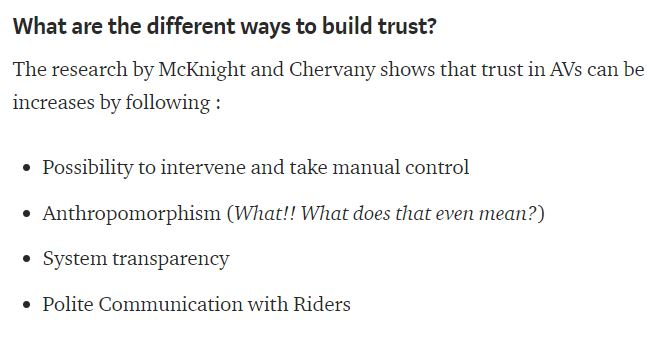
\includegraphics[width=0.734\columnwidth]{pictures/buildingTrust.jpg}
		\caption{nix}
		\label{img:buildingTrust}
	\end{figure}
	Stimme, Personalisierung von Assistenten im Fahrzeug\\
	Menschen und andere Autos auch im Navi darstellen; Die aktuell ausgeführte Situation als verschriftlicht anzeigen('beschleunige, Fußgänger im Weg, 400m zu Ziel')\\
	Anpassung des Autoinneren anhand der Person die einsteigt.\\
	Position des Autos auf der Straße anzeigen und den geplanten Weg\\
	\cite{b17}\\
	Ein 'Primärer Fahrer' ist bei Einstieg mehrere Personen zu identifizieren - damit es im Auto eine Person gibt, welche die Entscheidungen treffen wird. \cite{b18}; 'Communicate just enough';\\
	Userinterface sollte unterschiedlich designed sein, bei 'Luxusklasse', ggf sowas wie 'Kinderautos' oÄ\\
	Fahrassistent muss sich Personen im Auto anpassen.\\
	Gesammte Mensch-maschine Schnittstelle zu Konzept soll Anthropomorphistisch sein\\
	Steuerung und alles andere soll intuitiv aber auch allgegenwärtig sein\\
	
\end{itemize}

\begin{large}
	\textbf{Verkaufspsychologie, Designpsychologie und KISS noch ausschreiben!}\\
	
\end{large}

Verkauf: Verkaufspsychologische Meinungen hinzuziehen bei Preisbestimmung \& - optimierung.\\
Wirkung des Cockpits muss ansprechend wirken -> Designpsychologische Apskete beachten\\
KISS: alles muss in der am einfachsten \& verständlichsten Weise dargestellt werden\\
..? any more\\
Mögliche Orientierung an UCD-Ablauf Diagramm -> Josis Hausarbeit\\
Ressourcenauslastung: neben SW für autonome Fahrfunktionaöität müssen auf klassische Fahrassistenten onBoard sein die bei manueller STeuerung greifen\\
\subsection{Personas}
In meiner BA werde ich nur das männliche Geschlecht nutzen oder so -> Gendern wird misachtet\\
Bla, und so: AV sind sicherer als Menschen (Quelle suchen mit Unfall in \%)\\
Bla, hier wird jetzt das Forschungsseminar eingefügt.\\
Fahrzeugübergabe muss sicher sein (Wie übergebe ich ein FZ in einer Kurve?)\\
Ein Auto muss zuverlässig sein.	
Hier die KernElemente der WS sagen oder in der BA?